\documentclass[11pt,spanish,a4paper]{article}
% Versión 1.er cuat 2021 Víctor Bettachini < bettachini@df.uba.ar >

% Versión 1.er cuat 2021 Víctor Bettachini < bettachini@df.uba.ar >

\usepackage[T1]{fontenc}
\usepackage[utf8]{inputenc}

\usepackage[spanish, es-tabla]{babel}
\def\spanishoptions{argentina} % Was macht dass?
% \usepackage{babelbib}
% \selectbiblanguage{spanish}
% \addto\shorthandsspanish{\spanishdeactivate{~<>}}

\usepackage{graphicx}
\graphicspath{{./figuras/}}
% \usepackage{float}

\usepackage[arrowdel]{physics}
\newcommand{\pvec}[1]{\vec{#1}\mkern2mu\vphantom{#1}}
% \usepackage{units}
\usepackage[separate-uncertainty=true, multi-part-units=single, locale=FR]{siunitx}
\usepackage{isotope} % $\isotope[A][Z]{X}\to\isotope[A-4][Z-2]{Y}+\isotope[4][2]{\alpha}

\usepackage{tasks}
\usepackage[inline]{enumitem}
% \usepackage{enumerate}

\usepackage{hyperref}

% \usepackage{amsmath}
% \usepackage{amstext}
\usepackage{amssymb}

\usepackage{tikz}
\usepackage{tikz-dimline}
\usetikzlibrary{math}
\usetikzlibrary{arrows.meta}
% \usetikzlibrary{snakes}
% \usetikzlibrary{calc}
\usetikzlibrary{decorations.pathmorphing}
\usetikzlibrary{patterns}

\usepackage[hmargin=1cm,vmargin=1.6cm,nohead]{geometry}
% \voffset-3.5cm
% \hoffset-3cm
% \setlength{\textwidth}{17.5cm}
% \setlength{\textheight}{27cm}

\usepackage{lastpage}
\usepackage{fancyhdr}
\pagestyle{fancyplain}
\fancyhead{}
\fancyfoot{{\tiny \textcopyright DF, FCEyN, UBA}}
\fancyfoot[C]{ {\tiny Actualizado al \today} }
\fancyfoot[RO, LE]{Pág. \thepage/\pageref{LastPage}}
\renewcommand{\headrulewidth}{0pt}
\renewcommand{\footrulewidth}{0pt}


\begin{document}
\begin{center}
\textbf{Física 2} (Físicos) \hfill \textcopyright {\tt DF, FCEyN, UBA}\\
	\textsc{\LARGE N=2 grados de libertad forzados | Pulsaciones}
\end{center}

Los ejercicios con (*) entrañan una dificultad adicional. Son para investigar después de resolver los demás.



\begin{enumerate}


\documentclass[11pt,spanish,a4paper]{article}
% Versión 1.er cuat 2021 Víctor Bettachini < bettachini@df.uba.ar >

% Versión 1.er cuat 2021 Víctor Bettachini < bettachini@df.uba.ar >

\usepackage[T1]{fontenc}
\usepackage[utf8]{inputenc}

\usepackage[spanish, es-tabla]{babel}
\def\spanishoptions{argentina} % Was macht dass?
% \usepackage{babelbib}
% \selectbiblanguage{spanish}
% \addto\shorthandsspanish{\spanishdeactivate{~<>}}

\usepackage{graphicx}
\graphicspath{{./figuras/}}
% \usepackage{float}

\usepackage[arrowdel]{physics}
\newcommand{\pvec}[1]{\vec{#1}\mkern2mu\vphantom{#1}}
% \usepackage{units}
\usepackage[separate-uncertainty=true, multi-part-units=single, locale=FR]{siunitx}
\usepackage{isotope} % $\isotope[A][Z]{X}\to\isotope[A-4][Z-2]{Y}+\isotope[4][2]{\alpha}

\usepackage{tasks}
\usepackage[inline]{enumitem}
% \usepackage{enumerate}

\usepackage{hyperref}

% \usepackage{amsmath}
% \usepackage{amstext}
\usepackage{amssymb}

\usepackage{tikz}
\usepackage{tikz-dimline}
\usetikzlibrary{math}
\usetikzlibrary{arrows.meta}
% \usetikzlibrary{snakes}
% \usetikzlibrary{calc}
\usetikzlibrary{decorations.pathmorphing}
\usetikzlibrary{patterns}

\usepackage[hmargin=1cm,vmargin=1.6cm,nohead]{geometry}
% \voffset-3.5cm
% \hoffset-3cm
% \setlength{\textwidth}{17.5cm}
% \setlength{\textheight}{27cm}

\usepackage{lastpage}
\usepackage{fancyhdr}
\pagestyle{fancyplain}
\fancyhead{}
\fancyfoot{{\tiny \textcopyright DF, FCEyN, UBA}}
\fancyfoot[C]{ {\tiny Actualizado al \today} }
\fancyfoot[RO, LE]{Pág. \thepage/\pageref{LastPage}}
\renewcommand{\headrulewidth}{0pt}
\renewcommand{\footrulewidth}{0pt}


\begin{document}
\begin{center}
\textbf{Física 2} (Físicos) \hfill \textcopyright {\tt DF, FCEyN, UBA}\\
	\textsc{\LARGE Pulsaciones, batidos (o latidos, \emph{beats})}
\end{center}

Los ejercicios con (*) son opcionales.

\begin{enumerate}


\item \label{pendacop}
\begin{minipage}[t][2.2cm]{0.75\textwidth}
Considere el sistema de dos péndulos de igual longitud $l$ pero de masas diferentes $m_{a}$ y $m_{b}$, acoplados mediante un resorte
de constante $k$.
\end{minipage}
\begin{minipage}[c][2cm][t]{0.2\textwidth}
  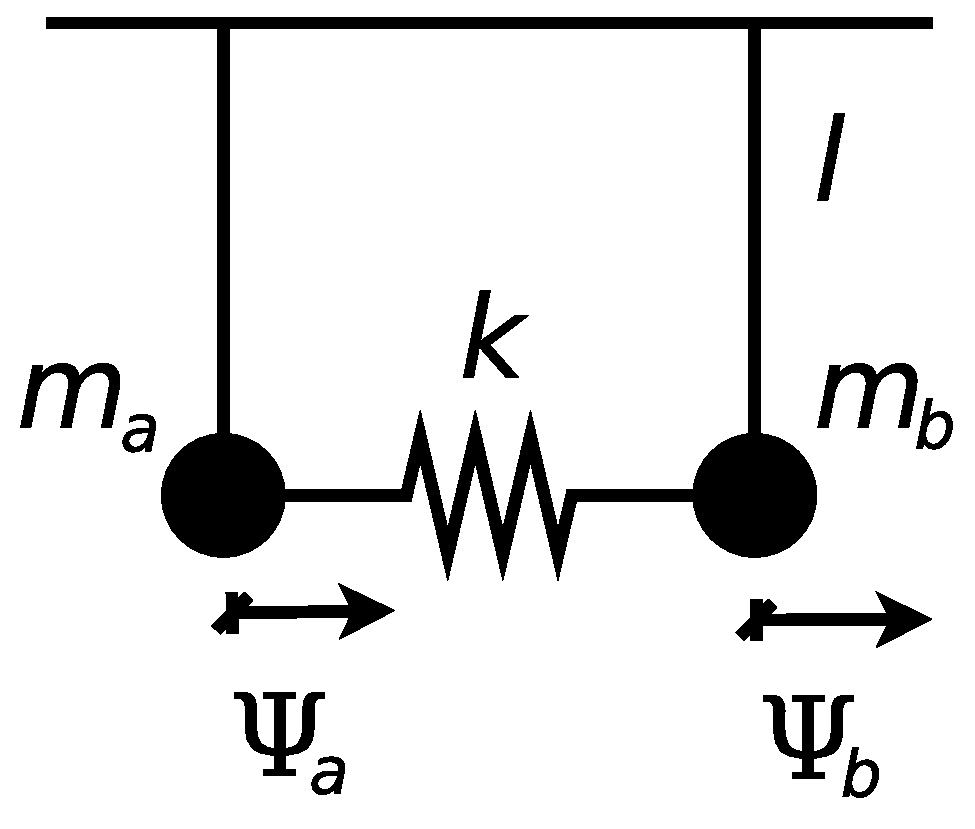
\includegraphics[width=\textwidth]{ej1-7}
\end{minipage}
\begin{enumerate}
	\item Escriba las ecuaciones de movimiento de cada masa. considerando pequeñas oscilaciones, ¿es relevante considerar $l_0\neq0$? ¿Qué cambia si el resorte es \emph{slinky}?   
	\item Obtenga las frecuencias naturales del sistema y sus modos normales de oscilación.
Interprete el significado físico de estos modos normales. 
	\item Suponga que el acoplamiento es débil ($k\ll\frac{g}{l}\frac{m_{a}m_{b}}{m_{a}+m_{b}}$) y que las condiciones iniciales son: $\dot{\Psi}_{a}(0)=0,\dot{\Psi}_{b}(0)=0,\Psi_{a}(0)=0,\Psi_{b}(0)=1$.
Obtenga el movimiento de cada masa y grafíquelo en función del tiempo.
	\item Calcule los valores medios, en un ciclo rápido, de $T_{a}$ y $T_{b}$, donde $T$ indica energía cinética. Grafique $\left\langle T_{a}\right\rangle $ y $\left\langle T_{b}\right\rangle $, y analice las diferencias en el gráfico como función de las diferencias entre las masas ($m_{a}=m_{b}$ y $m_{a}$ muy diferente de $m_{b}$).
Calcule el valor medio de la energía de interacción entre las dos partículas.
\end{enumerate}



\item \label{2masitas}
\begin{minipage}[t][2.8cm]{0.7\textwidth}
Considere el sistema de la figura. Las masas están apoyadas en una mesa sin rozamiento, sujetas a las paredes por resortes de constante
$k$ y unidas por otro resorte de constante $k'$.
\begin{enumerate}
	\item Obtenga las frecuencias y los modos transversales del sistema. 
	\item ¿Bajo qué condiciones espera observar batidos?
	¿Qué son los batidos?
\end{enumerate}
\end{minipage}
\begin{minipage}[c][0cm][t]{0.25\textwidth}
  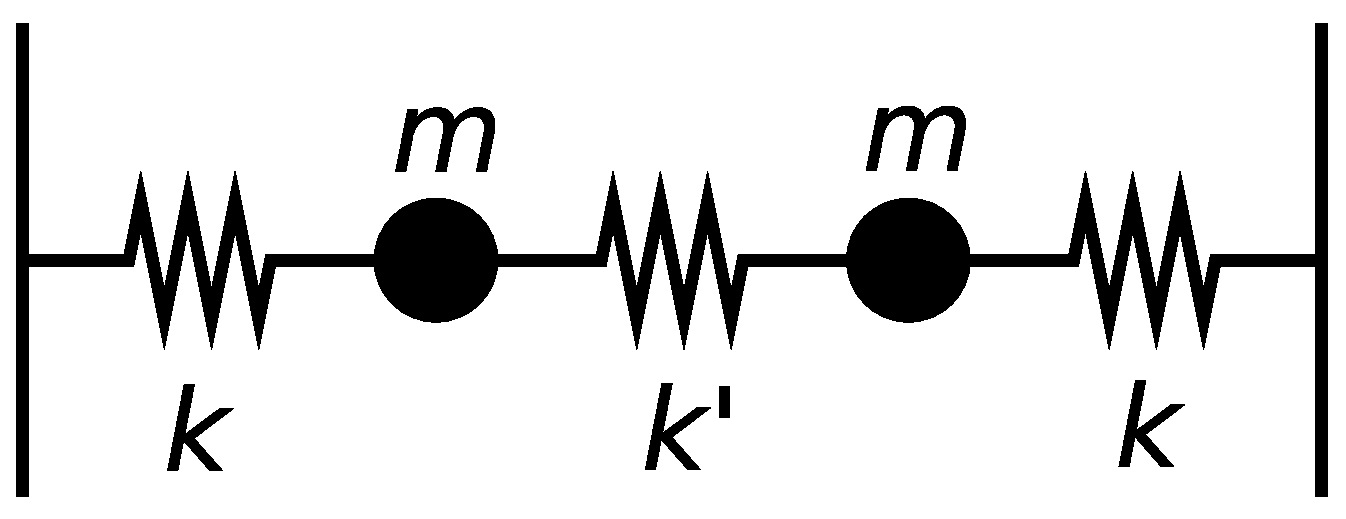
\includegraphics[width=\textwidth]{ej1-8}
\end{minipage}


\end{enumerate}

\end{document}

								
\subsection*{Sistemas de N grados de libertad forzados}


\item Considere el sistema de dos péndulos acoplados del problema \ref{pendacop}, tal que uno de ellos es impulsado por una fuerza $F= F_0 \cos(\Omega t)$.  
\begin{enumerate}
	\item Escriba las ecuaciones de movimiento del sistema con amortiguamiento y forzado y desacople las ecuaciones utilizando las coordenadas normales del sistema.
	\item Resuelva el sistema forzado para las coordenadas normales y luego escriba la solución más general posible para las coordenadas de las partículas a y b.
	\item Estudie el caso estacionario, observe cuando las partículas están en fase o contrafase.
	\item Muestre que considerando $m_a= m_b= m$ y despreciando el amortiguamiento se obtienen las siguientes expresiones.
		\begin{align}
			\Psi_a &\approx \frac{F_0}{2m} \cos(\Omega t) \left[ \frac{1}{\omega_1^2 - \Omega^2 } + \frac{1}{\omega_2^2 -\Omega^2} \right] \notag \\
			\Psi_b &\approx \frac{F_0}{2m} \cos(\Omega t) \left[ \frac{1}{\omega_1^2 - \Omega^2 } - \frac{1}{\omega_2^2 -\Omega^2} \right] \notag \\
			\frac{\Psi_b}{\Psi_a} &\approx \frac{\omega_2^2 - \omega_1^2}{\omega_2^2 + \omega_1^2 - 2 \Omega^2} \notag
		\end{align}
	donde $\omega_{1}$ es la menor de las frecuencias modales, $\omega_{2}$ es la mayor y $\Omega$ es la frecuencia de excitación.
	\item (*) Grafique $\frac{\Psi_b}{\Psi_a}$, ¿qué representa esta relación?
	Indique cuándo hay una transferencia efectiva de movimiento y cuándo no.
\end{enumerate}


\item Considere el sistema del problema \ref{2masitas}, pero en este caso en considere las oscilaciones longitudinales.
\begin{enumerate}
    \item Halle la solución estacionaria para el caso forzado en el cual se aplica sobre la masa de la izquierda una fuerza oscilante $F(t)= F_0 cos(\Omega t)$.
		¿Qué resonancias espera ver si realiza un barrido de frecuencias?
		\item (*) Repita el punto anterior, teniendo en cuenta además una fuerza de disipación proporcional a la velocidad
		\item (*) Repita el problema pero considerando las oscilaciones transversales del sistema
\end{enumerate}



%\item
%\begin{minipage}[t][3.5cm]{0.7\textwidth}
%Considere el sistema de 3 péndulos acoplados que se muestra en la figura.
%\begin{enumerate}
%	\item Escriba la ecuación de movimiento para cada masa y encuentre las frecuencias
%	propias y los modos normales del sistema. 
%	\item Suponga que en el extremo libre se aplica una fuerza $F= F_0 \cos(\omega t)$.
%	Escriba la ecuación de movimiento para cada masa y encuentre la solución estacionaria para cada modo.
%	¿Cuáles son las frecuencias de resonancia?
%\end{enumerate}
%\end{minipage}
%\begin{minipage}[c][0cm][t]{0.25\textwidth}
%  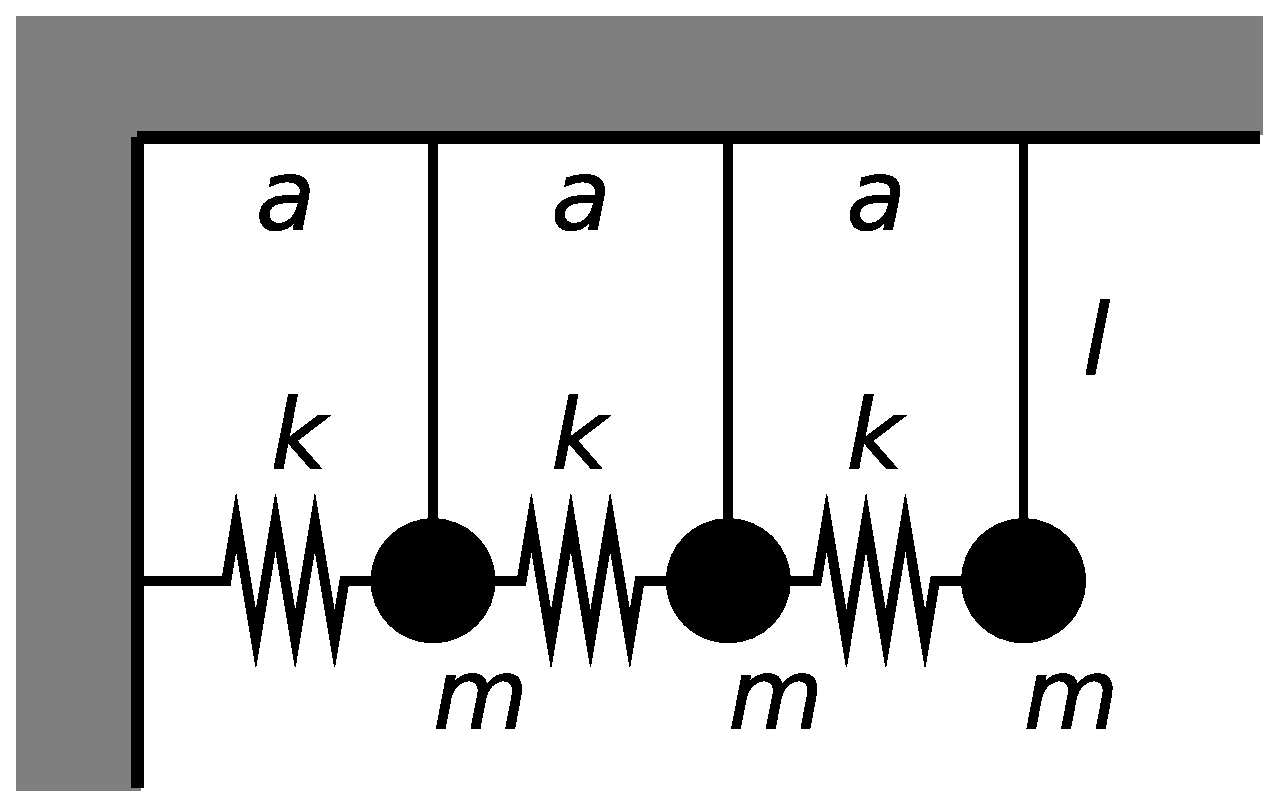
\includegraphics[width=\textwidth]{ej1-14}
%\end{minipage}



\end{enumerate}

\end{document}
